\subsection{Porovnanie prístupov}
Nakoniec by sme mali porovnať jednotlivé prístupy optimalizácie prevádzky zariadenia medzi sebou a zhodnotiť ich výhody aj nevýhody, i keď túto tematiku sme už načrtli pri hodnotení výsledkov daných metód.

Experiment bol postavaný podobne ako v predchádzajúcich častiach s tým rozdielom, že v tomto prípade sme experiment vykonali pre 50 rôznych realizácií šumu merania a výsledné riešenia spriemerovali. Rozptyl šumu merania sme nastavili pre koncentráciu biomasy $ W_{x} = 0.03\si{\gram\per\liter} $ a koncentráciu substrátu $ W_{s} = 0.025\si{\gram\per\liter} $. Pri schéme úpravy modifikátora sme nastavili váhový koeficient $ c = 0.8 $ a pri identifikácii FIR modelu sme zvolili chybu modelu rovnú rozptylu šumu merania $ \delta_{s} = 0.025\si{\gram\per\liter} $. Pri dvojkrokovej optimalizácii sme nastavili počiatočný nástrel odhadovaných parametrov nasledovne $ \mu_{m} = 0.5\si{\per\hour}, K_{M} = 1.0\si{\gram\per\liter}, K_{I} = 50.0\si{\gram\per\liter} $. Výsledok tohto porovnania môžeme vidieť na Obr. \ref{fig:method_comparison_bigNoise}, ktoré zobrazujú to isté a to priebeh výsledkov optimalizácie prevádzky zariadenia, ale každý obrázok v iných jednotkách. Na Obr. \ref{fig:method_comparison_costFunVal_bigNoise} sú vyjadrené rýchlosti riedenia v jednotlivých iteráciách z Obr. \ref{fig:method_comparison_D_bigNoise} ako hodnoty účelovej funkcie zariadenia, tak ako sme to zvykli zobrazovať doteraz. Na týchto obrázkoch sú zobrazené optimálne stavy zariadenia (bodkovaná čierna), nominálneho modelu (bodkovaná červená) a priebehy optimalizácie hybridným modelovaním (tyrkysová), schémou úpravy modifikátora (zelená) a dvojkrokovou optimalizáciou (modrá).
\begin{figure}
	\centering
	\begin{subfigure}[b]{0.49\textwidth}
		\centering
		\includegraphics[width=\linewidth]{images/method_comparison_costFunVal_bigNoise}
		\caption{Optimálne hodnoty $ D $ vyjadrené ako hodnota účelovej funkcie Monod modelu (zariadenia).}
		\label{fig:method_comparison_costFunVal_bigNoise}
	\end{subfigure}
	\hfill
	\begin{subfigure}[b]{0.49\textwidth}
		\centering
		\includegraphics[width=\linewidth]{images/method_comparison_D_bigNoise}
		\caption{Optimálne hodnoty rýchlosti riedenia $ D $. \newline \newline}
		\label{fig:method_comparison_D_bigNoise}
	\end{subfigure}
	\caption{Porovnanie priemerných výsledkov optimalizácie prevádzky zariadenia jednotlivých prístupov pri rôznych realizáciách šumu merania s rozptylom $ W_{x} = 0.03\si{\gram\per\liter} $ a $ W_{s} = 0.025\si{\gram\per\liter} $. Označenie \aps{PE} reprezentuje dvojkrokovú optimalizáciu, \aps{MAS} schéma úpravy modifikátora, \aps{HYB} hybridné modelovanie.}
	\label{fig:method_comparison_bigNoise}
\end{figure}

Dvojkroková optimalizácia sa vo väčšine prípadov v tretej iterácii  dostala do blízkosti optima zariadenia, ale v ďalších iteráciách divergovala. To je úplne odlišné správanie od toho, čo sme uviedli v predchádzajúcich výsledkoch dvojkrokovej optimalizácie a pôsobí veľmi nespoľahlivo, ak pre rôzne realizácie šumu získavame diametrálne odlišné výsledky. \textcolor{red}{Pravdepodobne, niektoré kombinácie parametrov, ktoré dobre aproximujú namerané údaje, vedú k odlišným optimám účelovej funkcie alebo príliš veľká hodnota $ K_{I} $ spôsobuje numerickú nestabilitu.}
 
Najlepšie z pomedzi týchto troch prístupov si viedla schéma úpravy modifikátora, ktorá nás vo väčšine prípadov posunula bližšie k optimu zariadenia. Jasnou nevýhodou je, že vo väčšine prípadov je konvergencia veľmi pomalá a to môže byť veľký problém ak jedna iterácia trvá hodiny alebo dni, ako v našom prípade. Ďalšou nevýhodou je, že potrebujeme údaje o ustálenom stave koncentrácie biomasy a tá sa bežne ani nemeria, a keď aj áno, tak s veľkým rozptylom chyby merania. V princípe, by sme mohli tieto údaje odhadovať, ale odhad stavov je vždy založený na matematickom modely, ktorý je v našom prípade nepresný, čo by v spojení s fluktuáciou chyby merania viedlo k veľmi nepresným odhadom. 

Ako sme už uviedli v predchádzajúcej časti, hybridné modely definované rovnicami \eqref{eq:hybrid_opt_bio} a \eqref{eq:hybrid_opt_subs} nie sú vhodné na statickú optimalizáciu, pretože týmto prístupom nedokážu upraviť gradient účelovej funkcie natoľko, aby sme skonvergovali k optimálnemu chodu zariadenia. Ale na rozdiel od schémy úpravy modifikátora majú jednu veľkú výhodu a tou je predikcia údajov. Vďaka tejto vlastnosti sa môžu využiť na riadenie, a keďže dynamiku nominálneho modelu upravujeme pomocou dátových modelov na základe nameraných údajov zo zariadenia, dokážeme dosiahnuť omnoho lepšie výsledky v oblasti riadenia ako so samotným nominálnym modelom.

Porovnanie predikčných vlastností a dynamiky zariadenia, nominálneho a hybridného modelu môžeme vidieť na Obr. \ref{fig:hybrid_dynamics_comparison}. Údaje na identifikáciu FIR modelu sme získali využitím schémy úpravy modifikátora. Tú sme nechali bežať do ôsmej iterácie, kde dosiahla rýchlosť riedenia $ D = 0.3821\si{\per\hour} $. Trénovacie údaje sú zobrazené na Obr. \ref{fig:hybrid_dynamics_data}, kde môžeme vidieť aj výstup identifikovaného FIR model 3. rádu. Aby sme dosiahli nižší rád modelu, museli sme zväčšiť chybu modelu na $ \delta_{s} = 0.05\si{\gram\per\liter} $. Aby sme otestovali predikciu hybridného modelu, zvolili sme si tri rôzne rýchlosti riedenia. Dve také, ktoré boli zahrnuté v dátach na trénovanie modelu a jednu novú, optimálnu rýchlosť riedenia nášho zariadenia, ktorá už v dátach obsiahnutá nebola. Je zrejmé, že predikcia hybridného modelu je omnoho lepšia ako predikcia samotného nominálneho modelu. Ak testovacie dáta boli obsiahnuté v dátach na trénovanie, teraz máme na mysli $D = \lbrace D_{N}^{\star}, 0.385 \rbrace\si{\per\hour} $, tak výstup z hybridného modelu dokázal veľmi presne odhadnúť skutočný výstup zo zariadenia. Na druhej strane, ak sme mu ponúkli ešte nepoznané vstupné dáta, vznikla nám odchýlka, ktorá je stále menšia ako odchýlka nominálneho modelu od zariadenia. Z tohto dôvodu si dovolíme tvrdiť, že v oblasti riadenia by hybridné modely našli omnoho väčšie uplatnenie ako pri statickej optimalizácii.

\begin{figure}
	\centering
	\begin{subfigure}[b]{0.49\textwidth}
		\centering
		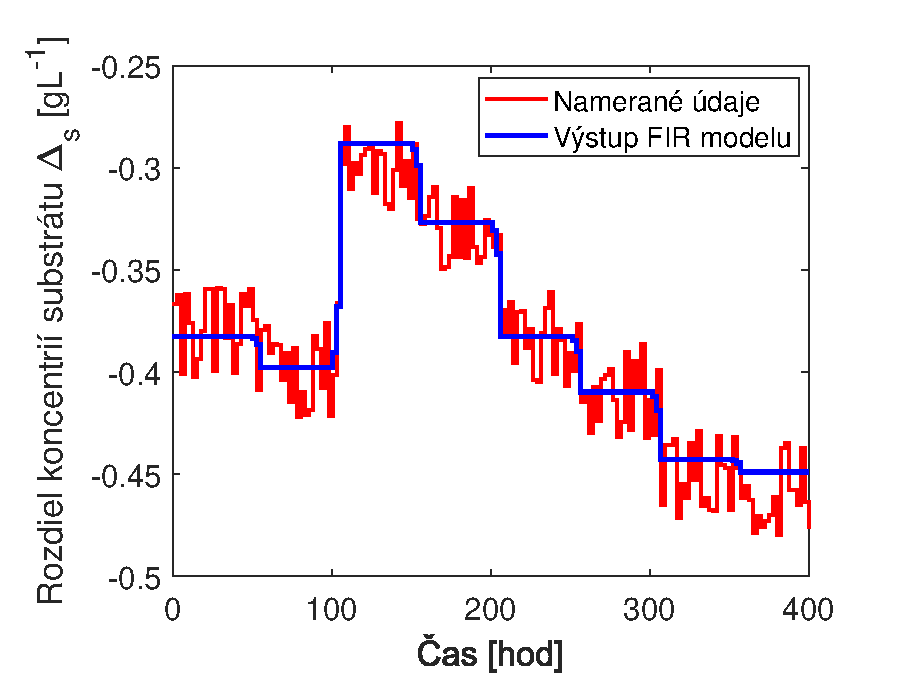
\includegraphics[width=\linewidth]{images/hybrid_dynamics_data}
		\caption{Trénovacie údaje. \newline}
		\label{fig:hybrid_dynamics_data}
	\end{subfigure}
	\hfill
	\begin{subfigure}[b]{0.49\textwidth}
		\centering
		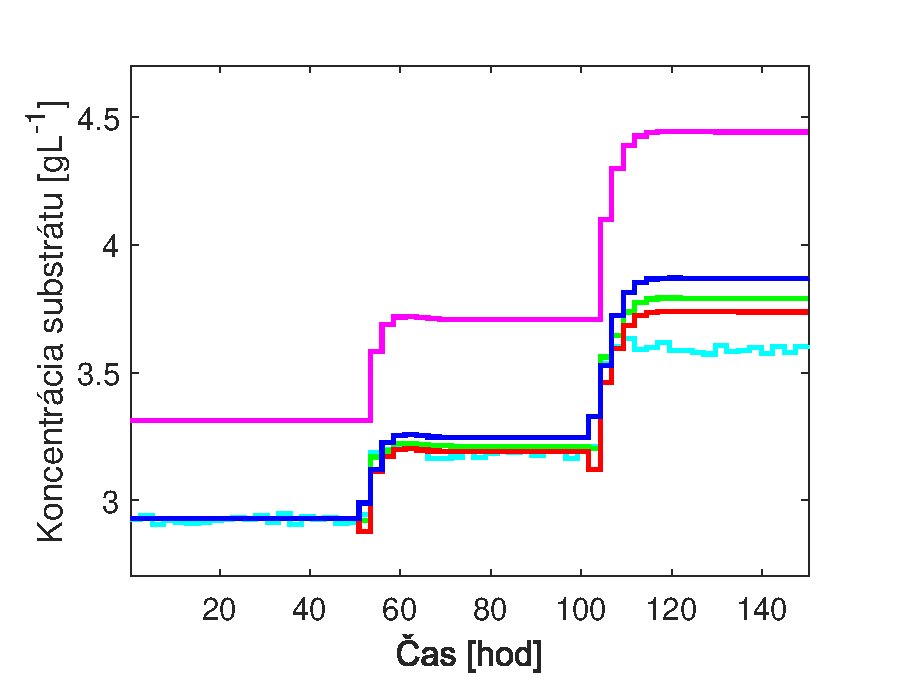
\includegraphics[width=\linewidth]{images/hybrid_dynamics_comparison}
		\caption{Porovnanie dynamiky a predikcie modelov.}
		\label{fig:hybrid_dynamics_comparison}
	\end{subfigure}
	\caption{Porovnanie predikčných schopností nominálneho a hybridného modelu, ktorý bol identifikovaný pomocou dát získaných schémou úpravy modifikátora. Testovacie vstupné údaje boli $ D = \lbrace D_{N}^{\star}, 0.385, D_{P}^{\star} \rbrace \si{\per\hour} $.}
	\label{fig:hybrid_dynamics_and_prediction}
\end{figure}

